\section{Load Balancing}
% 5 pages
% a little bit on the history of load-balancing, what types of technique are there? What are the different levels, why do we need level 7?, etc. etc.

\subsection{ Definition \& Role In a Typical Serverless Framework}
First, we want to discuss what component exactly we mean by \textit{load balancer}, and how it functions in the context of a serverless framework. While our approach is not tied to any specific serverless framework, implementation, or technology, we developed it with their general concepts and functioning in mind. Because of this we feel that is helpful and informative to explain the components of our system in the context of an actual implementation, since this helps understand the abstract role these components play. In addition this is helpful for anyone who might want to integrate our approach into a production ready serverless edge computing platform.

As previously mentioned there are a number of different serverless frameworks, some free, some open source, some commercial, and some that fall in-between\cite{aws-lambda}\cite{azure-functions} \cite{openfaas-gateway}\cite{kubeless}\cite{openwhisk}.
We choose OpenFaaS\cite{openfaas}
as our reference implementation of a serverless framework because it is open source, allowing us detailed understanding of its inner workings, because it has been extended, for edge computing, and because it builds on and makes use of well established technologies in the same way other serverless frameworks do\cite{kubeless}\cite{openwhisk}, thus making it representative for the space.


\begin{figure}
    \centering
    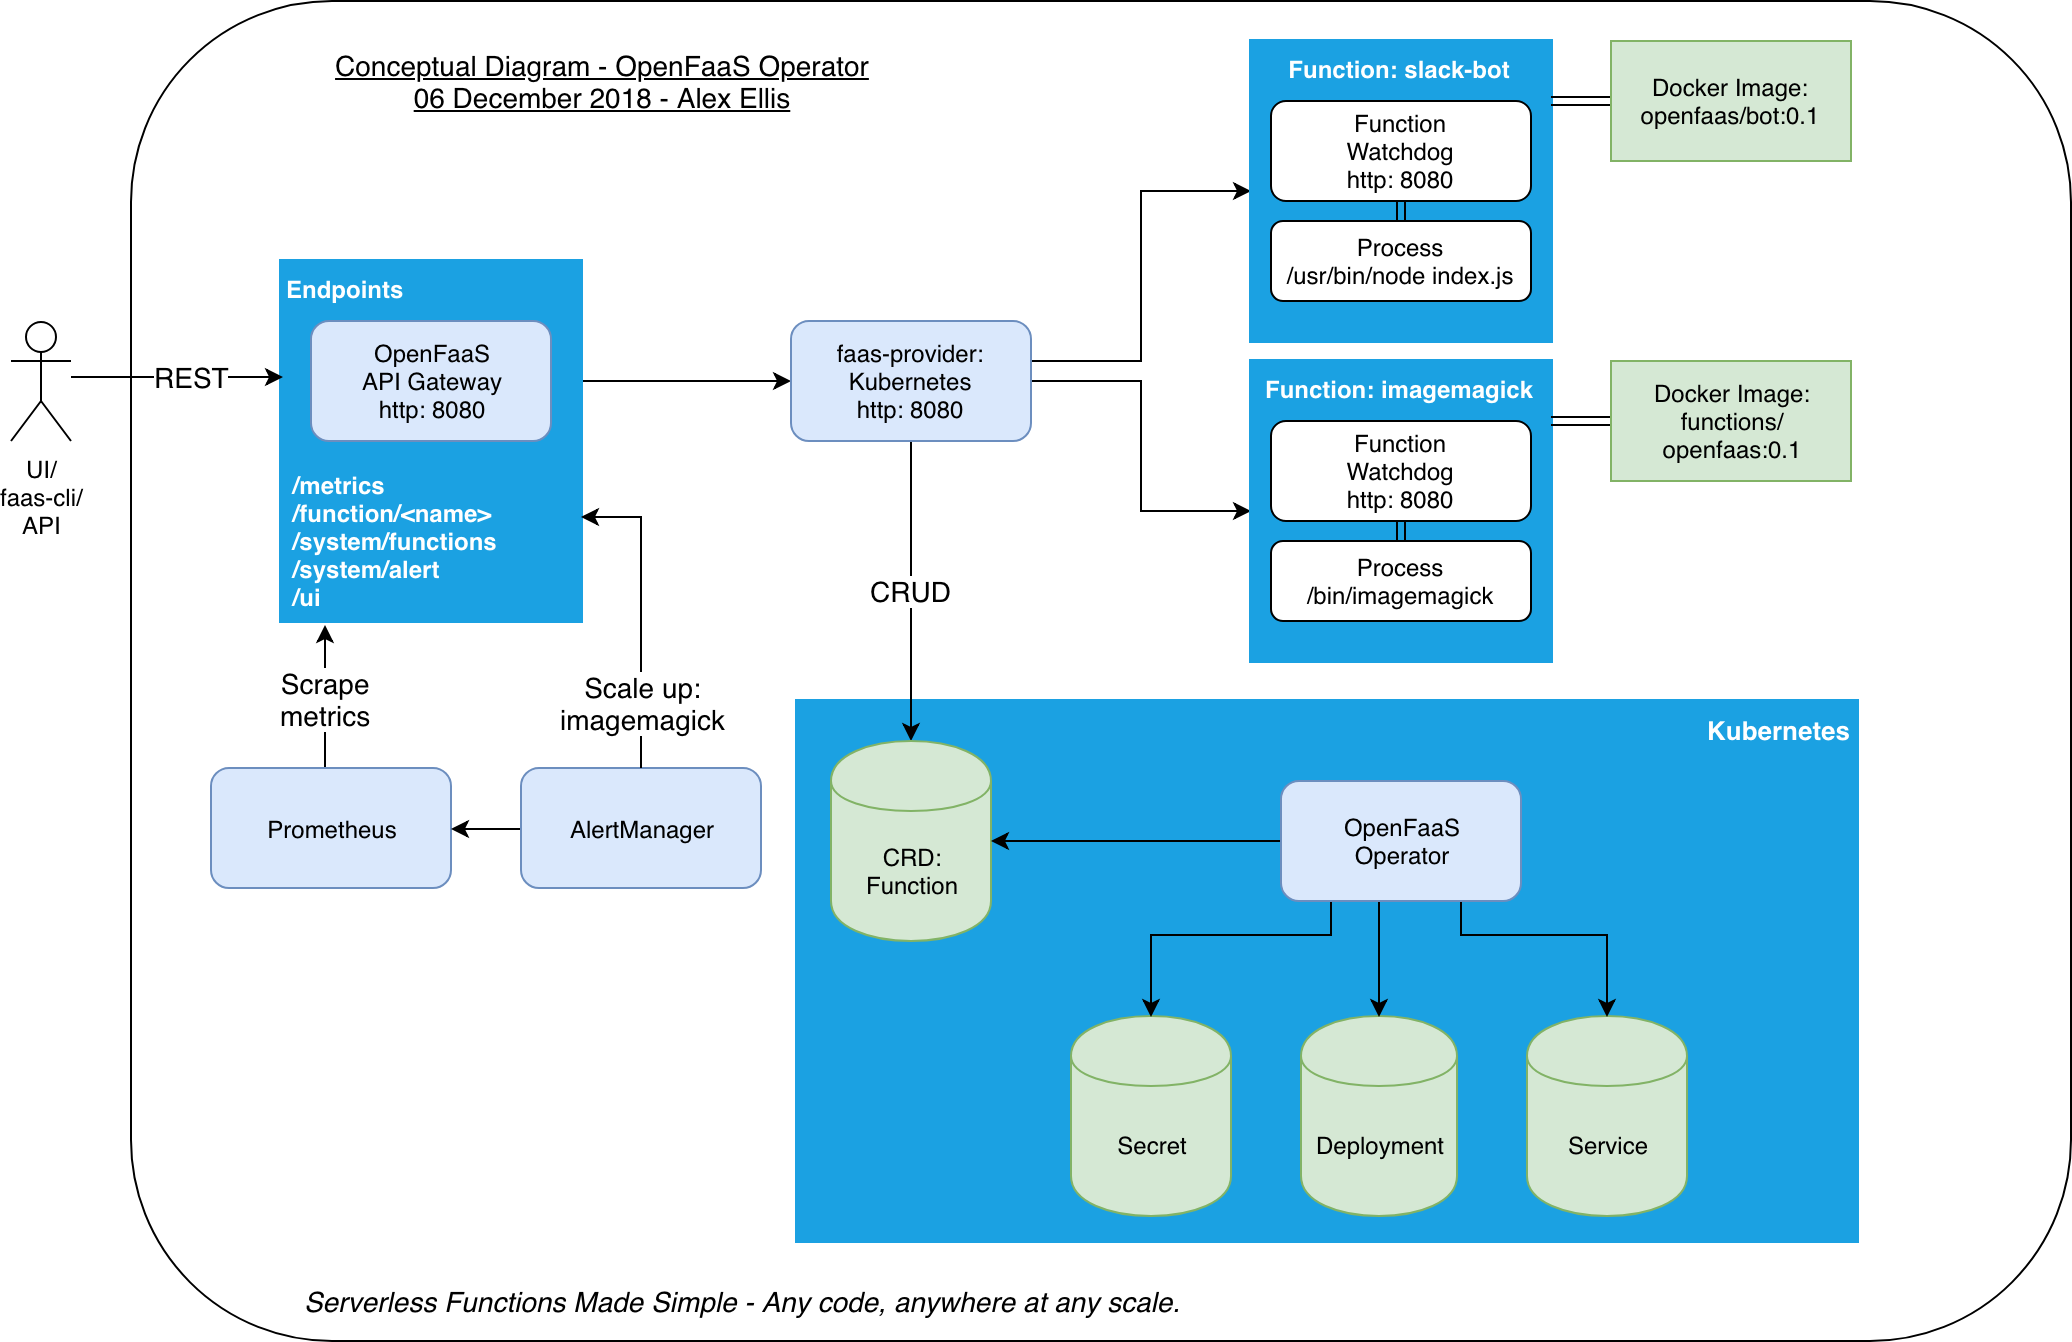
\includegraphics[width=14cm]{graphics/diagrams/openfaas-gateway-architecture.png}
    \caption{Diagram showing the architecture and components of OpenFaaS, in particular the OpenFaaS API Gateway. Taken from the official OpenFaaS architecture documentation\cite{openfaas-gateway}}
    \label{fig:openfaas-gateway-diagram}
\end{figure}


As mentioned, OpenFaaS uses Linux containers to run functions, and in turn Kubernetes to manage these containers. To clarify the role our load balancer would take in a serverless system, we describe how it would affect OpenFaaS. By default OpenFaaS employs a component they call \textit{API Gateway}. This API Gateway is the component which first receives \textbf{all} client requests, and then continues to send them on to the corresponding functions, while at the same time collecting metrics used by the system for tasks like auto-scaling. Figure \ref{fig:openfaas-gateway-diagram}, which is taken directly from the official OpenFaaS documentation shows the interactions with the other components of the system. Since the API Gateway is just another container running in Kubernetes\cite{kubernetes}, and failover capability is a concern, there can be multiple instances of the API Gateway running at any given time.
As discussed a major reason for the sub-optimal performance of network bound workloads in edge scenarios is the lack of efficient request routing.
In the case of OpenFaaS this stems from it delegating networking and routing tasks to Kubernetes, since it is the underlying container orchestration platform. This applies to both the initial ingress into the cluster, as well as to how the API Gateway forwards client requests to the relevant replicas to be processed. Kube-proxy, the component of Kubernetes which handles networking and routing tasks, will default to the round-robin policy of selecting upstreams. While it is possible to set up kube-proxy in a way that will prefer nodes in the same zone based on a label, this functionality is built around cloud based deployments and is insufficient to address the heterogeneity in networking and compute power introduced by edge computing. This defaulting to round-robin means that in effect, serverless frameworks such as OpenFaaS route the requests basically at random between the entry point in the network and the API Gateway, and then from the API Gateway to the relevant function.\\
In our approach the load balancer takes the role the API Gateway has in OpenFaaS. It is characterized by being
\begin{enumerate}
    \item the entry point for the client to the serverless system, meaning there are no network hops between the load balancer instance and the node the request originally arrived at, and
    \item directly forwarding requests to the corresponding serverless function instances.
\end{enumerate}
When implementing our proposed approach in practise this would mean that the serverless framework would have to be adapted to fulfill these conditions for the load balancer. If these conditions aren't met, this would likely negate the positive affect our approach has on performance.

As an example in the case of OpenFaaS, referencing the OpenFaaS architecture in Figure \ref{fig:openfaas-gateway-diagram}, this could be realized in the following ways:
\begin{enumerate}
    \item API Gateways and load balancers are scaled and scheduled together, meaning they are always co-located on the same node. The API-Gateway would then still first receive requests and handle implementation specific tasks for the serverless system, but then forward the request to the load balancer instance on the same node, which then decides on further request routing.
    \item The load balancer is the new entry point for clients, effectively replacing the API Gateway. In this scenario the load balancer and API Gateway would also be altered such that metrics and information relevant to the system could be collected by the load balancers and forwarded to API Gateway instances, which then handle them as before.
\end{enumerate}